\section{Evaluation von Klassifikationen}

Beim maschinellen Lernen ist die Bewertung ein wichtiger Schritt f�r die Auswahl eines Klassifizierungsalgorithmus. Diese Auswertung erfolgt anhand von Testdaten, die nicht f�r das Training verwendet wurden. Ein guter Indikator f�r die G�te eines Klassifikators ist die Anzahl der Testdatens�tze, die der Klassifikator richtig und falsch klassifiziert hat. Dies l�sst sich am besten durch eine Konfusionsmatrix veranschaulichen.

\subsection{Evaluation mittels Konfusionsmatrix}

Bei einer Klassifikationsaufgabe, bei der Datens�tze von \(n\) Klassen \(K_1, \ldots, K_n\) klassifiziert werden, wird folgendes durchgef�hrt:
\begin{enumerate}
    \item Unter Verwendung der Klassen \(K_1, \ldots, K_n\) wird eine Matrix \(M\) konstruiert.
    \item In den diagonalen Feldern (\(K_i, K_i\)) von M wird die Anzahl der korrekt klassifizierten Datens�tze eingetragen.
    \item In den Feldern (\(K_r, K_s\)) wobei \(r \neq s\) wird die Anzahl der falsch klassifizierten Datens�tze eingetragen.
\end{enumerate}

\subsection{Konfusionsmatrix f�r zwei Klassen}

Die Datens�tze bestehen aus zwei Klassen \(K_p = \) Positive und \(K_n = \) Negative. Aus dem Datensatz wird die folgende Konfusionsmatrix konstruiert:

\begin{figure}[H]
    \centering
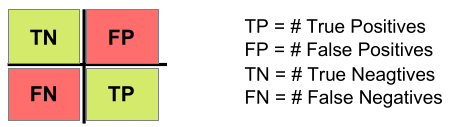
\includegraphics[width=0.6\textwidth]{figures/kap12/2-class-confusion-matrix.png}
    \caption{Konfusionsmatrix f�r zwei Klassen}
    \label{fig:confusion-matrix-2-class}
\end{figure}


Aus dieser Konfusionsmatrix kann das Folgende f�r Klasse \(K_p\) berechnet werden:

\begin{itemize}
    \item Precision, P: \[P = \frac{TP}{TP + FP}\]
    \item Recall, R: \[R = \frac{TP}{TP + FN}\]
    \item Specifity, S: \[S = \frac{TN}{FP + TN}\]
    \item \(F_1\textnormal{-Ma�}\), \(F_1\): \[F_1 = \frac{2*TP}{2*TP+FP+FN}\]
    \item Matthews Correlation Coefficient \[MCC = \frac{TP \times TN - FP \times FN }{\sqrt{(TP+FP)(TP+FN)(TN+FP)(TN+FN)}}\]
\end{itemize}

\subsection{Bewerstungsma�e f�r Klassifikatoren, die numerische Scores liefern}

Einige Klassifikationsaufgaben liefern numerische Werte mit einem Wert von 0 bis 1. Die Idee zur Bewertung dieser Art von Klassifikator besteht darin, die Abweichung der vom Klassifikator erhaltenen Bewertungen im Vergleich zu den tats�chlichen Bewertungen f�r den Datensatz zu berechnen. Es gibt zahlreiche Kennwerte, die auf diesem Prinzip beruhen:

\begin{itemize}
    \item Mittlerer Quadratischer Fehler (MSE): \[MSE = \frac{(p_1 - a_1)^2 + \ldots + (p_n - a_n)^2}{n}\]
    \item Wurzel aus MSE (RMSE): \[RMSE = \sqrt{\frac{(p_1 - a_1)^2 + \ldots + (p_n - a_n)^2}{n}}\]
\end{itemize}

\section{Fehlerquellen f�r maschinelles Lernen}

\begin{itemize}
    \item \textbf{Overfitting:} �beranpassung tritt auf, wenn ein Modell zu gut f�r die Trainingsdaten trainiert wurde. W�hrend des Trainings, um die besten Ergebnisse des Klassifikators beim Testen zu erhalten, wurde m�glicherweise die Varianz eines wichtigen Merkmals �bersch�tzt. Wenn dies geschieht, kann der Klassifikator beim Testen als sehr genau bewertet werden, wird aber neue Daten falsch klassifizieren.
    \item \textbf{Modelle mit Bias:} Ein Modell wird biased, wenn der zum Trainieren des Modells verwendete Datensatz nicht repr�sentativ f�r die tats�chliche Aufgabe war. Das kann viele Ursachen haben, vielleicht wurden Daten aus der falshen Zielgruppe verwendet, oder es wurden nur Profile mit einem bestimmten Feature genommen oder vielleicht war ein Sensor bei der Erfassung der Daten defekt.
    \item \textbf{Overfitting plus Bias:} Wenn ein Klassifikator mit mehreren Datens�tzen trainiert wird und die Leistung der Klassifikatoren gemessen wird, sollte es keine gro�e Varianz geben. Wenn die Varianz hoch ist, bedeutet dies, dass der Klassifikator stark auf kleine �nderungen in den Daten reagiert.
\end{itemize}